\chapter{Metodologia}
\label{cap:metodologia}

Nesse capítulo serão abordados os métodos de pesquisa de juízes \textit{online} e os métodos de desenvolvimento do GOJ. Os critérios para seleção de juízes \textit{online}, os métodos de contagem de seus problemas, a arquitetura geral e do GOJ e a arquitetura e tecnologias utilizadas em cada um dos módulos do sistema.

\section{Pesquisas de juízes online}

Nessa seção serão descritos os métodos para levantamento do número de questões e das funcionalidades em juízes \textit{online} selecionados, além disso, serão apresentados os critérios de seleção dos juízes.

\subsection{Critérios de seleção de juízes}
\label{subsec:selecao_juizes}

Define-se juiz \textit{online} como um site ou página que armazena questões e possibilita ao usuário enviar submissões dessas questões, para serem testadas e um veredicto seja retornado. Foi realizada uma seleção de juízes \textit{online} com base em pesquisas de termos no \textit{Google}\footnote{\url{https://www.google.com/}}, mecanismo de pesquisas \textit{online}. Para a seleção de resultados foram considerados apenas os sites que se encaixam no termo juiz \textit{online}, conforme definido anteriormente. As buscas englobam as páginas 1 e 2 de pesquisa e cada busca teve diferentes resultados, que serão listados, com base nos termos pesquisados. Os itens estão enumerados em ordem de relevância, determinada pelo mecanismo de pesquisa que lista os resultados mais relevantes primeiro, ou seja, os itens estão em ordem de aparição. Vale ressaltar que durante as buscas o mecanismo de pesquisa oferece páginas como anúncio, porém, os anúncios da ferramenta de pesquisa não foram considerados nas escolhas, apenas os outros sites resultado das buscas.

A primeira busca realizada foi com o termo em inglês ``\textit{Online judge}'', que teve os seguintes resultados:

\begin{enumerate}
    \item OnlineJudge
    \item Beecrowd
    \item Sphere Online Judge (SPOJ)
    \item PKU JudgeOnline
\end{enumerate}

Esses foram os juízes listados com o termo ``\textit{Online judge}'': o Online Judge\footnote{\url{https://www.onlinejudge.org/}}, um juiz \textit{online} também conhecido como \textit{UVa}, que teve seu nome alterado recentemente;
o Beecrowd\footnote{\url{https://www.beecrowd.com.br}}, que também é conhecido como URI,  também teve seu nome e endereço alterados recentemente; 
o Sphere Online Judge (SPOJ)\footnote{\url{https://www.spoj.com/}}; e o PKU JudgeOnline\footnote{\url{http://poj.org/}} um juiz \textit{online} da Universidade de Pequim.

O segundo termo pesquisado foi o termo em inglês ``\textit{Online programming contests}'', e os resultados foram:

\begin{enumerate}
    \item CodeChef
    \item Google's Coding Competitions
    \item Beecrowd
    \item Sphere Online Judge (SPOJ)
    \item Hackerearth
\end{enumerate}

O novo termo foi pensando em sites que, além de realizarem a função de juiz \textit{online}, possuem competições de programação; com isso, temos alguns novos juízes diferentes dos da busca anterior, são eles: CodeChef\footnote{\url{https://www.codechef.com/}}, um juiz \textit{online} com competições e que também armazena questões para práticas posteriores; Goolge's Coding Competitions\footnote{\url{https://codingcompetitions.withgoogle.com/}}, site onde estão reunidos links para competições do Google como Kick Start\footnote{\url{https://codingcompetitions.withgoogle.com/kickstart/about/}}, Hash Code\footnote{\url{https://codingcompetitions.withgoogle.com/hashcode/about/}} e CodeJam\footnote{\url{https://codingcompetitions.withgoogle.com/codejam/about/}}; e por fim, o Hackerearth\footnote{\url{https://www.hackerearth.com/}}, site muito usado para validação técnica de candidatos em entrevistas de emprego.

O terceiro termo pesquisado foi ``\textit{Programming competitions and contests}'', e os resultados foram:

\begin{enumerate}
    \item Google's Coding Competitions
    \item CodeChef
    \item Codeforces
    \item Hackerearth
\end{enumerate}

A ideia do terceiro termo é ressaltar sites de competição e o único site novo que apareceu foi o Codeforces\footnote{\url{https://codeforces.com/}}, um site mais voltado para competições, e que tem um vasto número de problemas para práticas posteriores.

O quarto termo pesquisado foi ``juiz \textit{online} programação'', e os resultados foram:

\begin{enumerate}
    \item Beecrowd
    \item Neps Academy 
    \item CodeBench
\end{enumerate}

A ideia do termo é tentar encontrar juízes \textit{online} com questões em português, ou até mesmo o suporte brasileiro. Com o primeiro termo em português obteve-se 2 novos resultados: Neps Academy\footnote{\url{https://neps.academy/}}, um site voltado para o ensino de programação, com aulas e questões para treino; e o CodeBench\footnote{\url{https://codebench.icomp.ufam.edu.br/}}, site voltado para ensino, com criação de turma e inscrição de alunos. 

Também foram pesquisados os termos ``programação'' e``\textit{contests} de programação'', porém, não foram encontrados novos resultados, apenas os já citados: Beecrowd e Neps Academy.

\subsection{Levantamento do número de problemas}
\label{subsec:levantamento_numero_de_problemas}

Dentre os juízes selecionados na Subseção \ref{subsec:selecao_juizes}, foi realizado um levantamento do número total de problemas de cada um deles. Para isso, distintas abordagens foram escolhidas com base no juiz \textit{online}. Nessa subseção serão apresentadas as abordagens e estratégias utilizadas para a contagem de problemas.

Para o levantamento dos problemas da plataforma Online Judge foi acessado a aba \textit{Browse Problems}\footnote{\url{https://onlinejudge.org/index.php?option=com\_onlinejudge\&Itemid=8}}, conforme disposto na Figura \ref{fig:online_judge_1}, e em cada umas das categorias, foi contado o número de problemas presentes, demonstrado na Figura \ref{fig:online_judge_2}. Para contagem do número de problemas, foi utilizado um \textit{script} em linguagem de programação \textit{python}, disponível no Apêndice \ref{appendix:script_oj}, com a estratégia de localizar o padrão em links de categorias e links de problemas. O primeiro padrão observado é que as pastas ficam em uma tabela; ao localizar a tabela pelo \textit{HTML} da página, é possível encurtar a busca pelos links. O segundo padrão que vale ressaltar é que os problemas possuem o trecho ``\texttt{page=show\_problem}'' na \textit{(URL)}, e isso diferencia um link de outra pasta para o link de um problema.

\begin{figure}[H]
    \centering
    \caption{Online Judge — Browse Problems}
    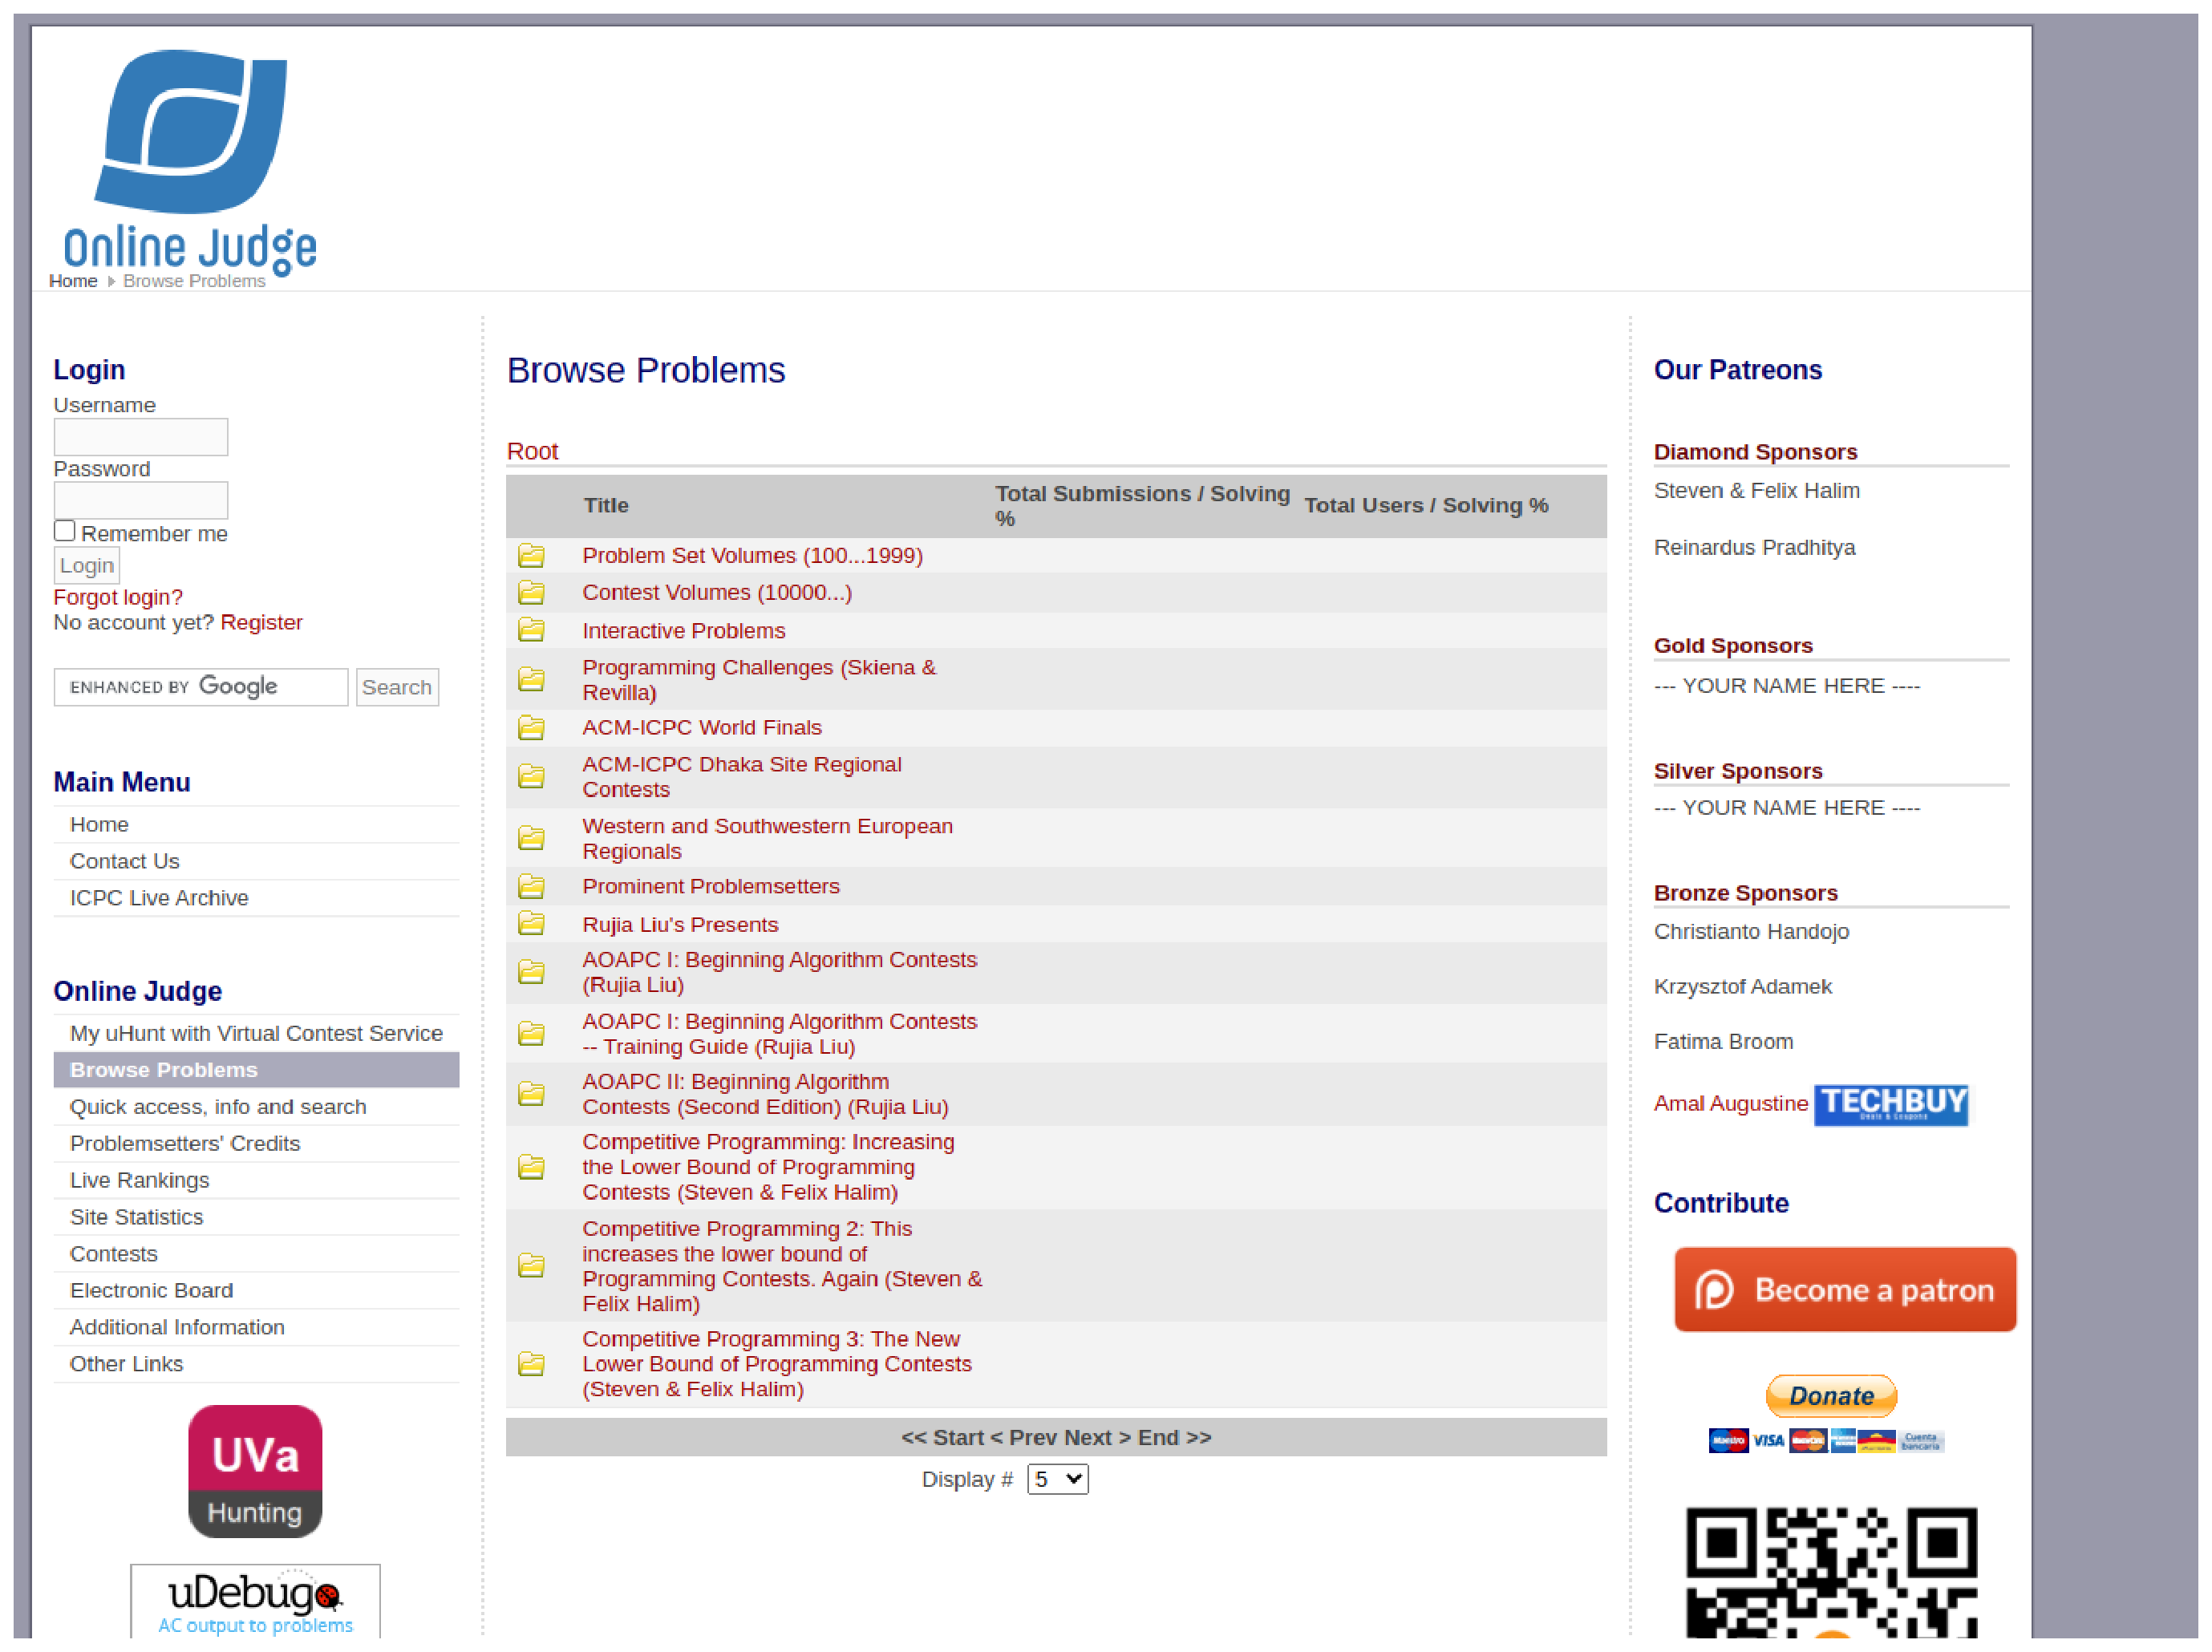
\includegraphics[keepaspectratio=true,scale=0.32]{figuras/online_judge_1.eps}
    \label{fig:online_judge_1}
\end{figure}

\begin{figure}[H]
    \centering
    \caption{Online Judge — Browse Problems (Detalhes)}
    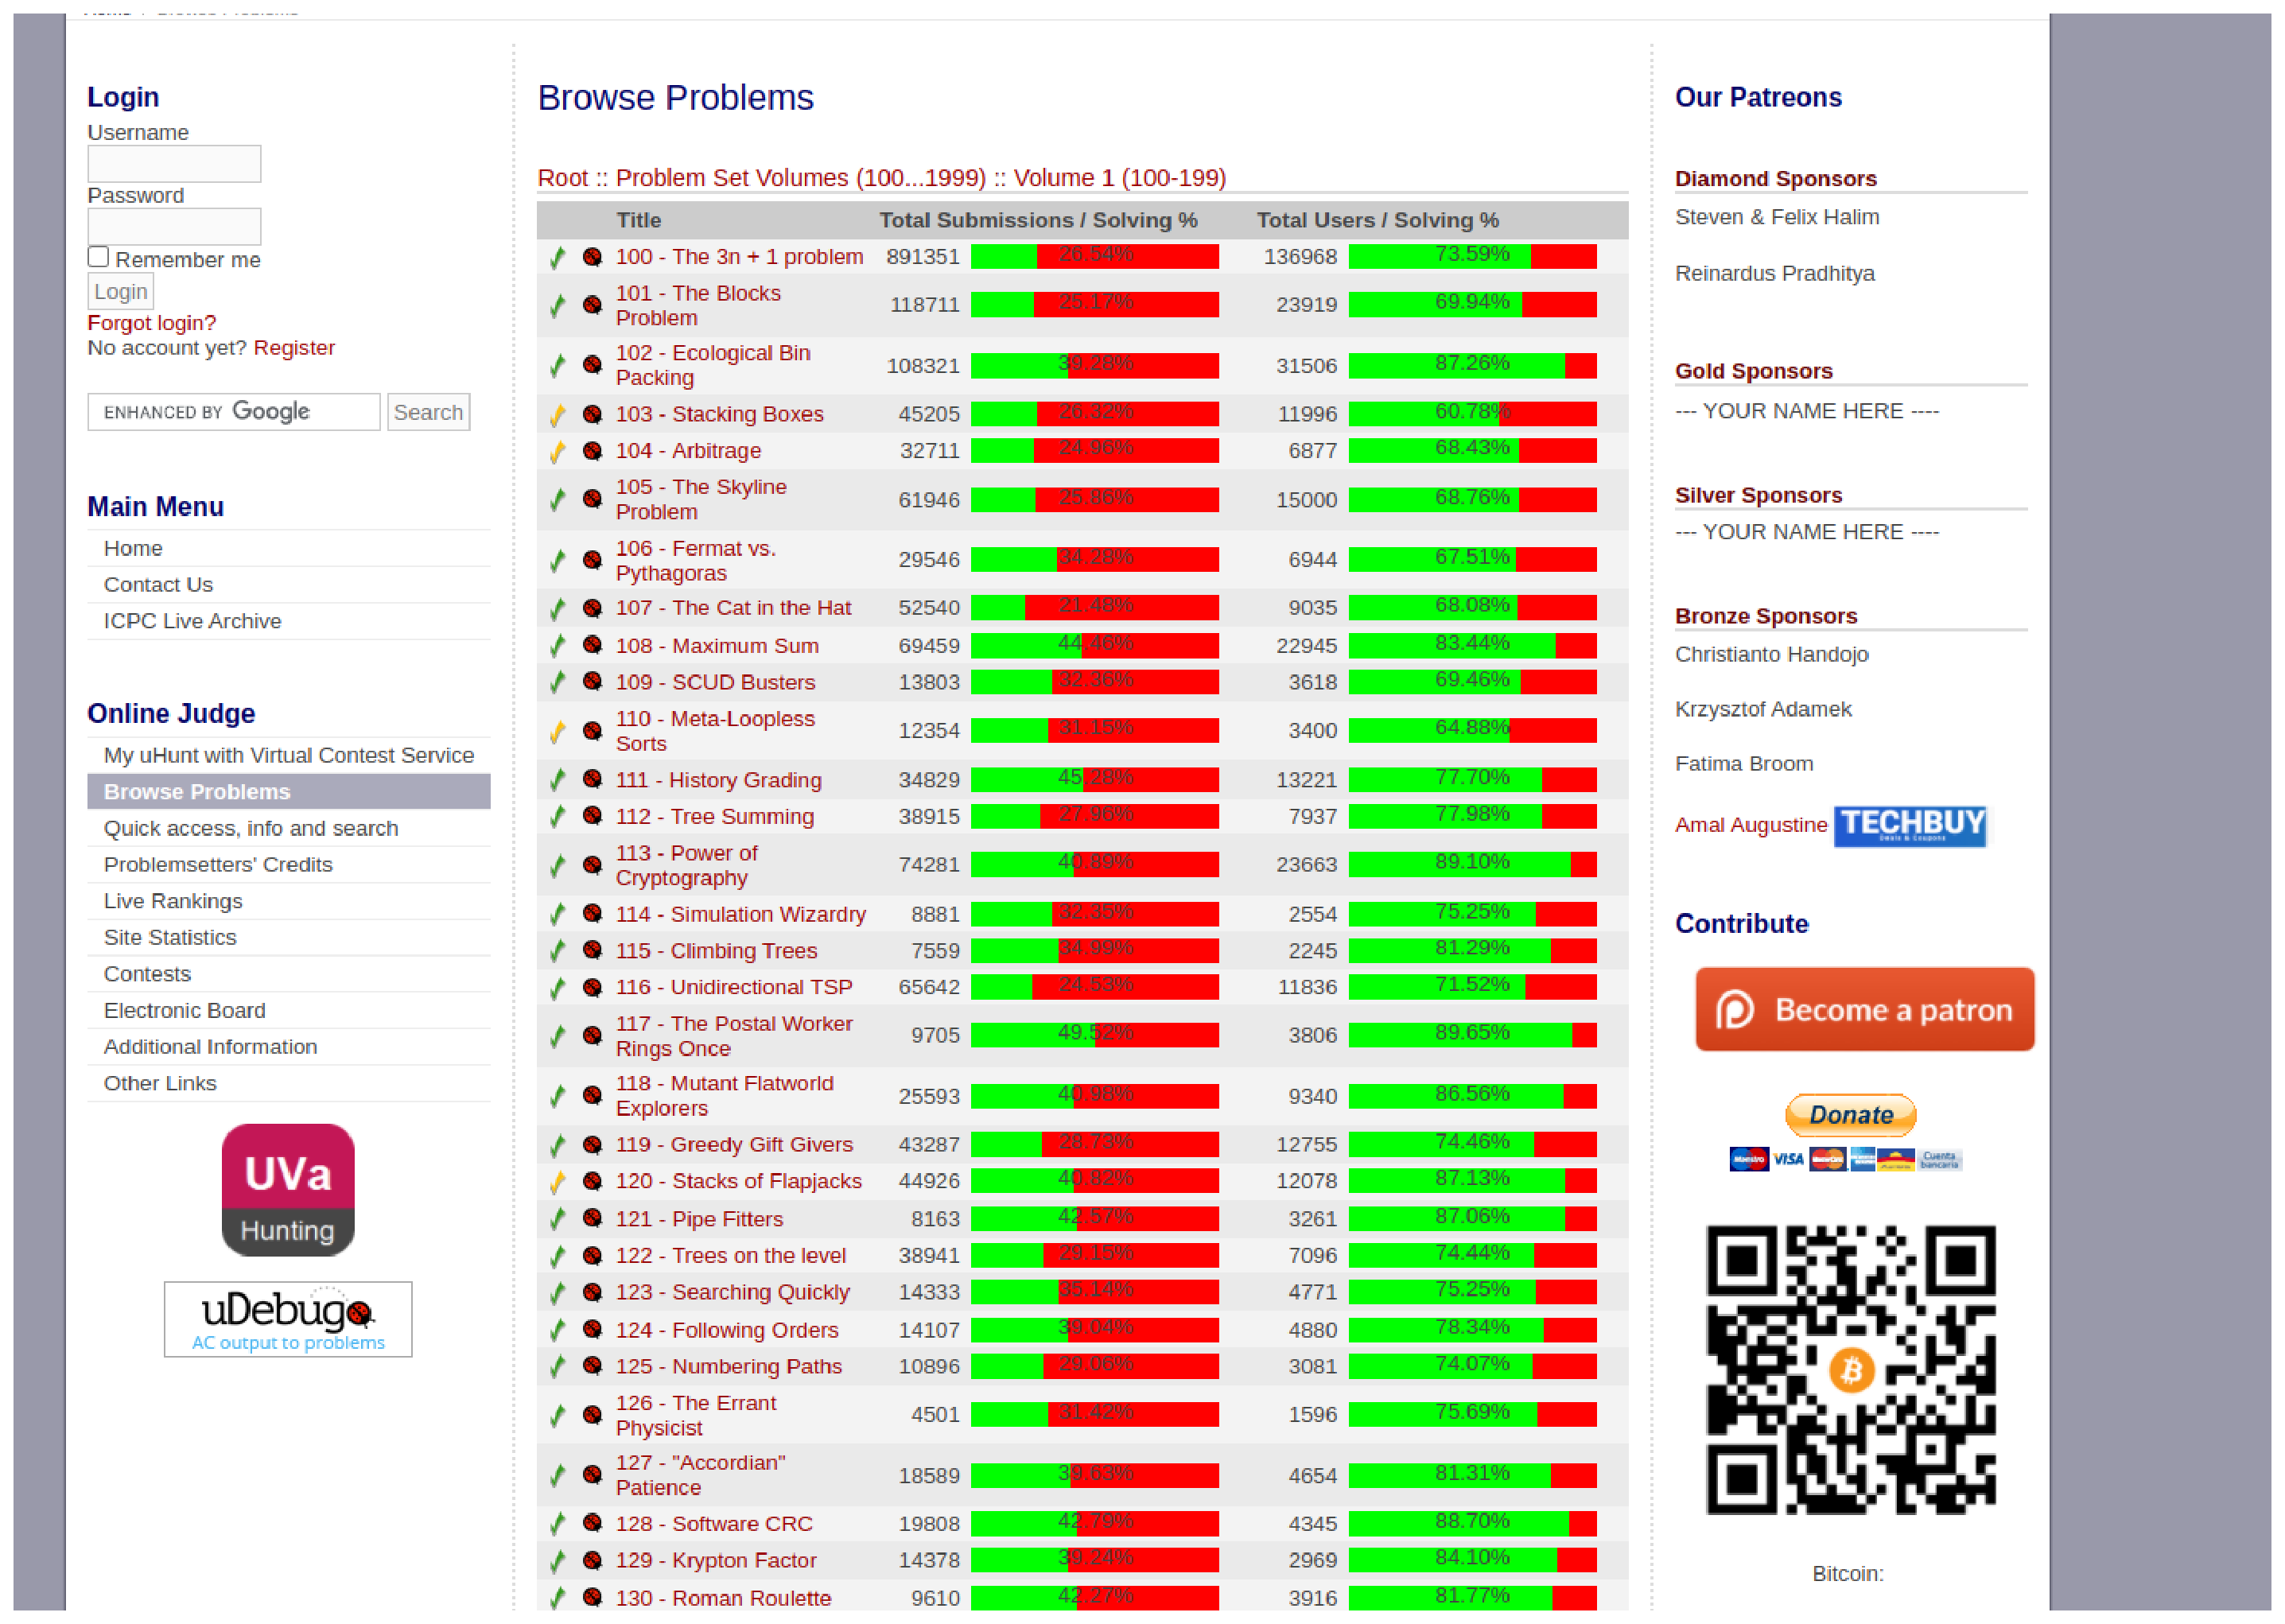
\includegraphics[keepaspectratio=true,scale=0.32]{figuras/online_judge_2.eps}
    \label{fig:online_judge_2}
\end{figure}

No site Beecrowd, foi preciso acessar a \textit{URL} de categorias\footnote{\url{https://www.beecrowd.com.br/judge/pt/categories}} e o número de problemas é exibido na categoria ``Listar todos''. Conforme apresentado na Figura \ref{fig:beecrowd_1}, o texto da opção ``Listar todos'' apresenta o número total de problemas da plataforma.

\begin{figure}[H]
    \centering
    \caption{Beecrowd — Total de problemas}
    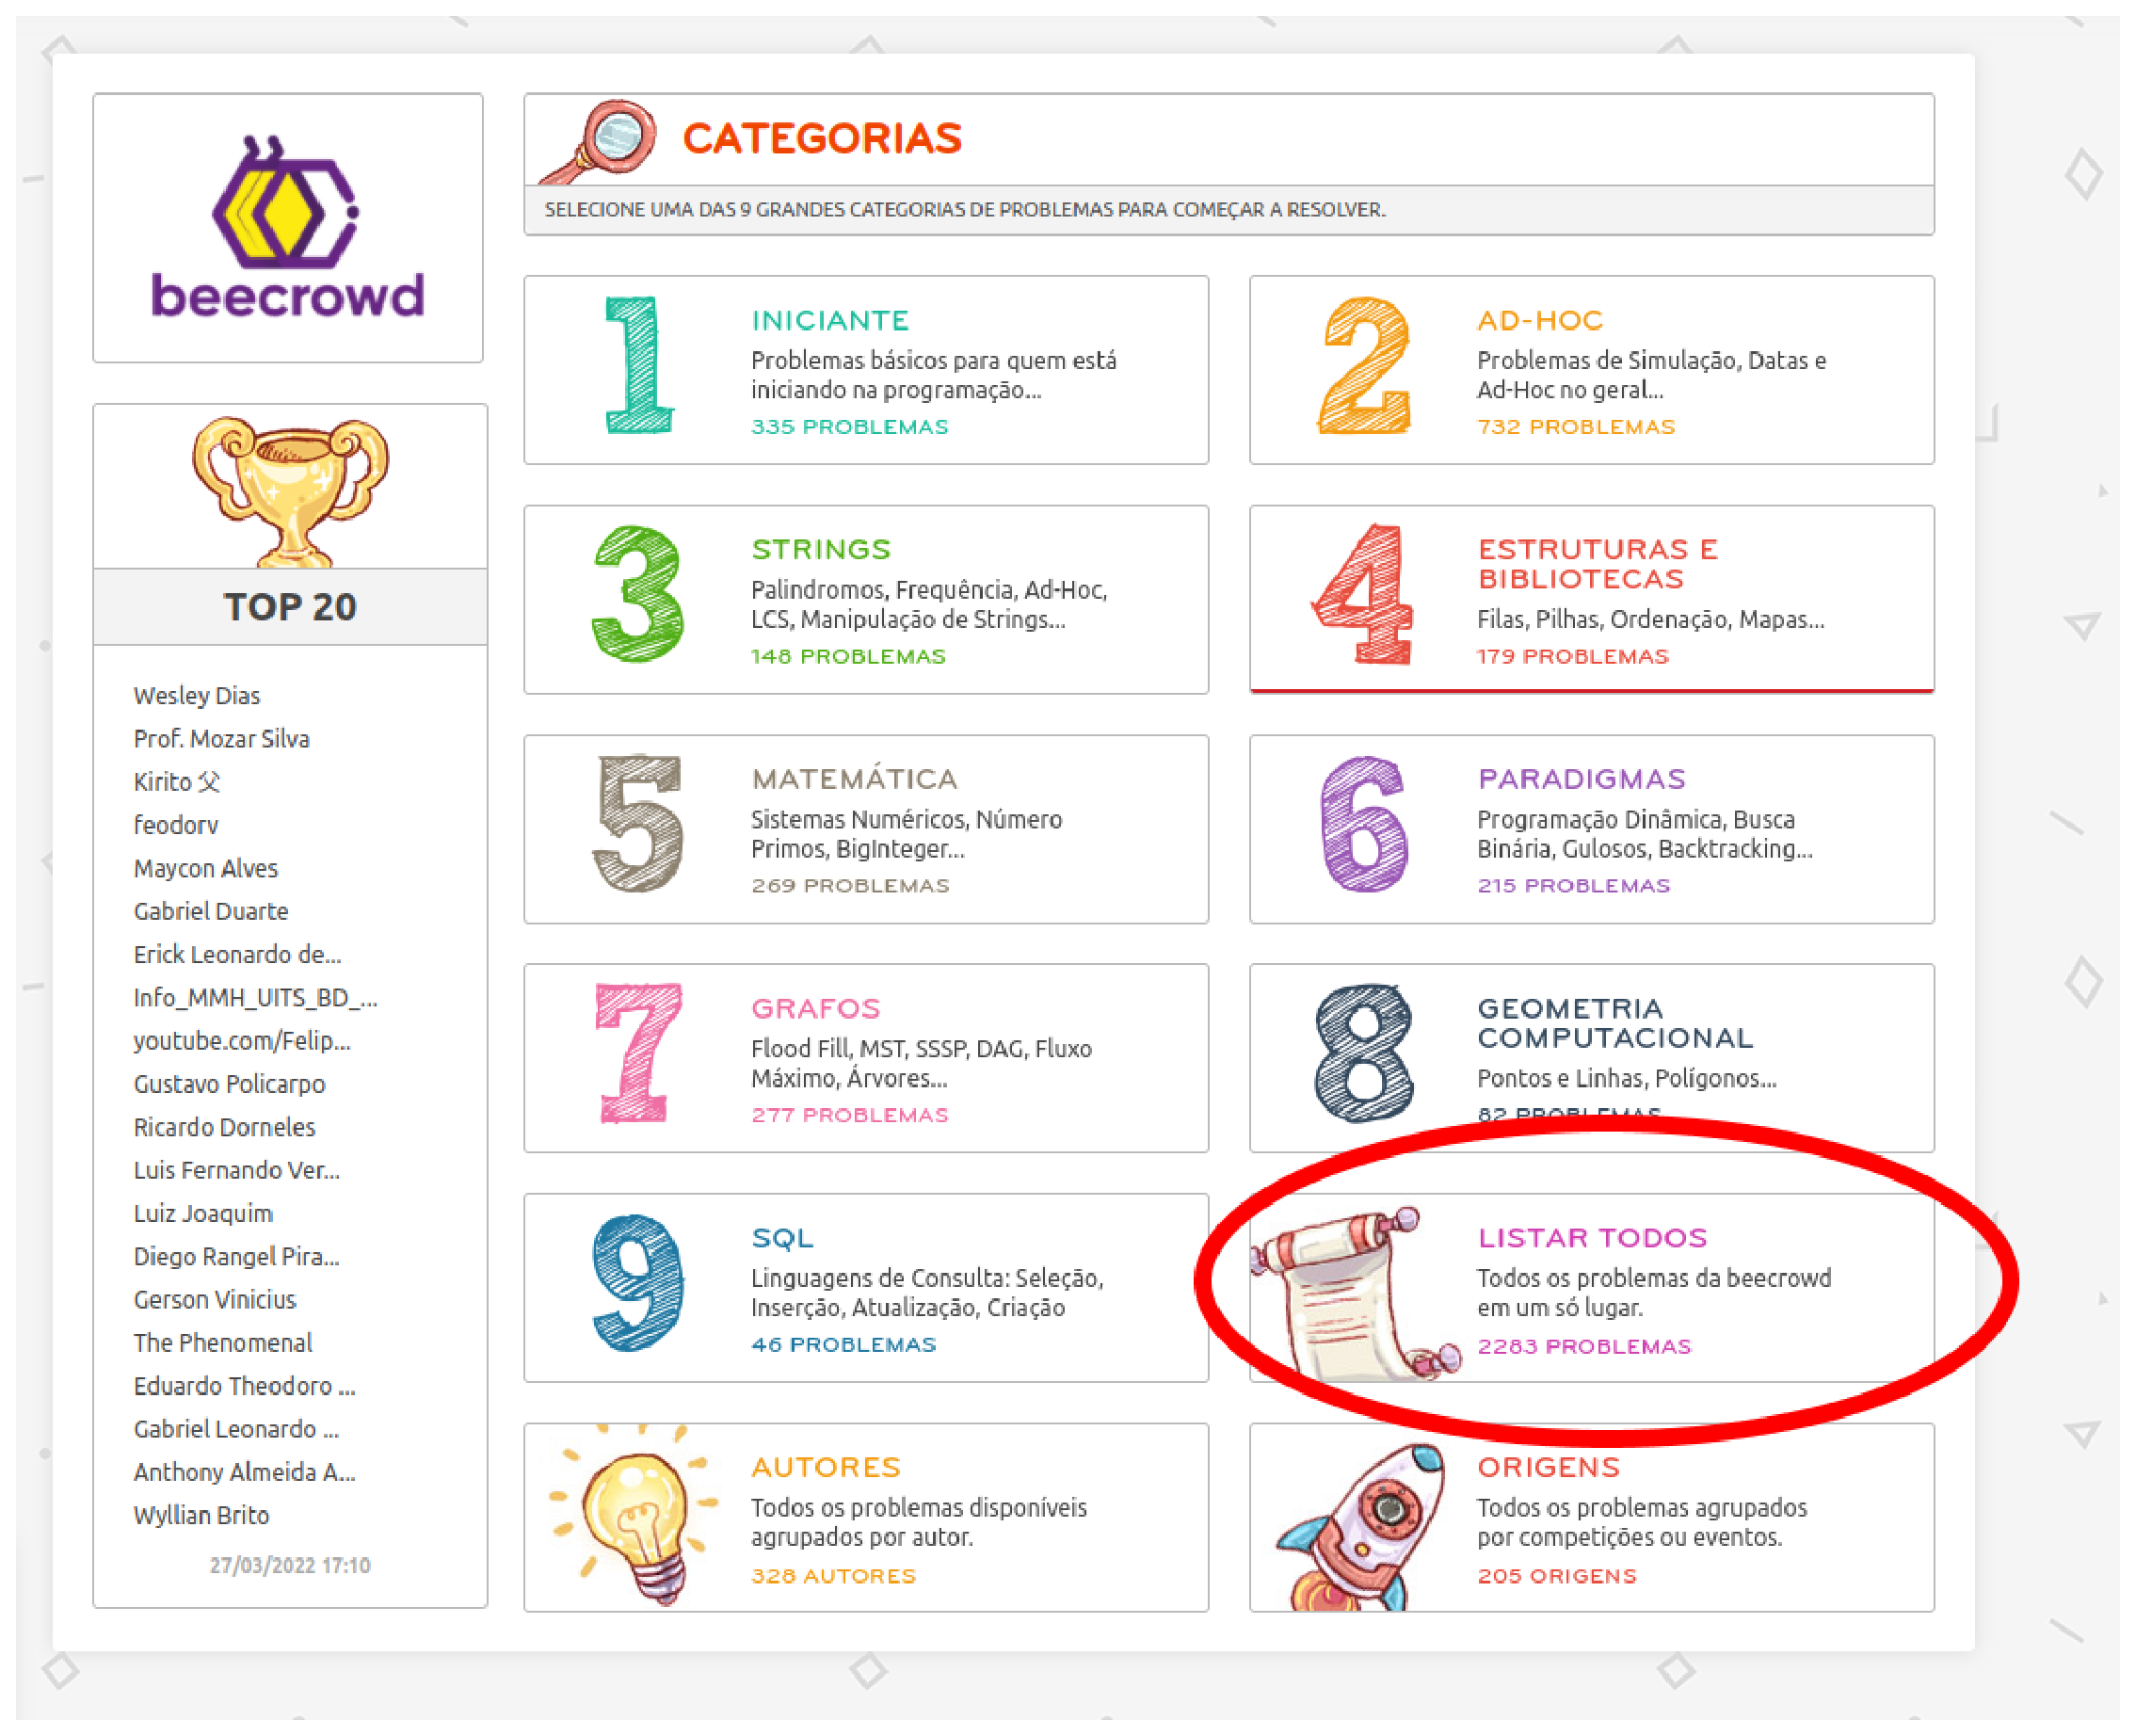
\includegraphics[keepaspectratio=true,scale=0.4]{figuras/beecrowd_1.eps}
    \label{fig:beecrowd_1}
\end{figure}

No Codeforces, foi utilizado a \textit{API} pública do site\footnote{\url{https://codeforces.com/apiHelp}}, que possui recursos para acessar as informações da plataforma; A \textit{API} é acessada via protocolo \textit{HTTP} e possui \textit{endpoints} públicos e privados. Um dos \textit{endpoints} públicos é para visualização das informações dos problemas, que retorna todos os problemas quando nenhum filtro é informado. Para recuperação do número total de problemas foi utilizado um \textit{script} em linguagem \textit{bash}, disponível no Apêndice \ref{appendix:script_cf}.

Para o levantamento no site Code Chef, foi acessada a página de problemas do site, e dentro dela, utilizou-se o filtro \textit{``All Levels''} que revelou os problemas de todos os níveis, como apresentado na Figura \ref{fig:code_chef_1}. Com isso, foi possível observar o número de problemas mais abaixo, conforme demonstra a Figura \ref{fig:code_chef_2}.

\begin{figure}[H]
    \centering
    \caption{Code Chef — Filtro de problemas}
    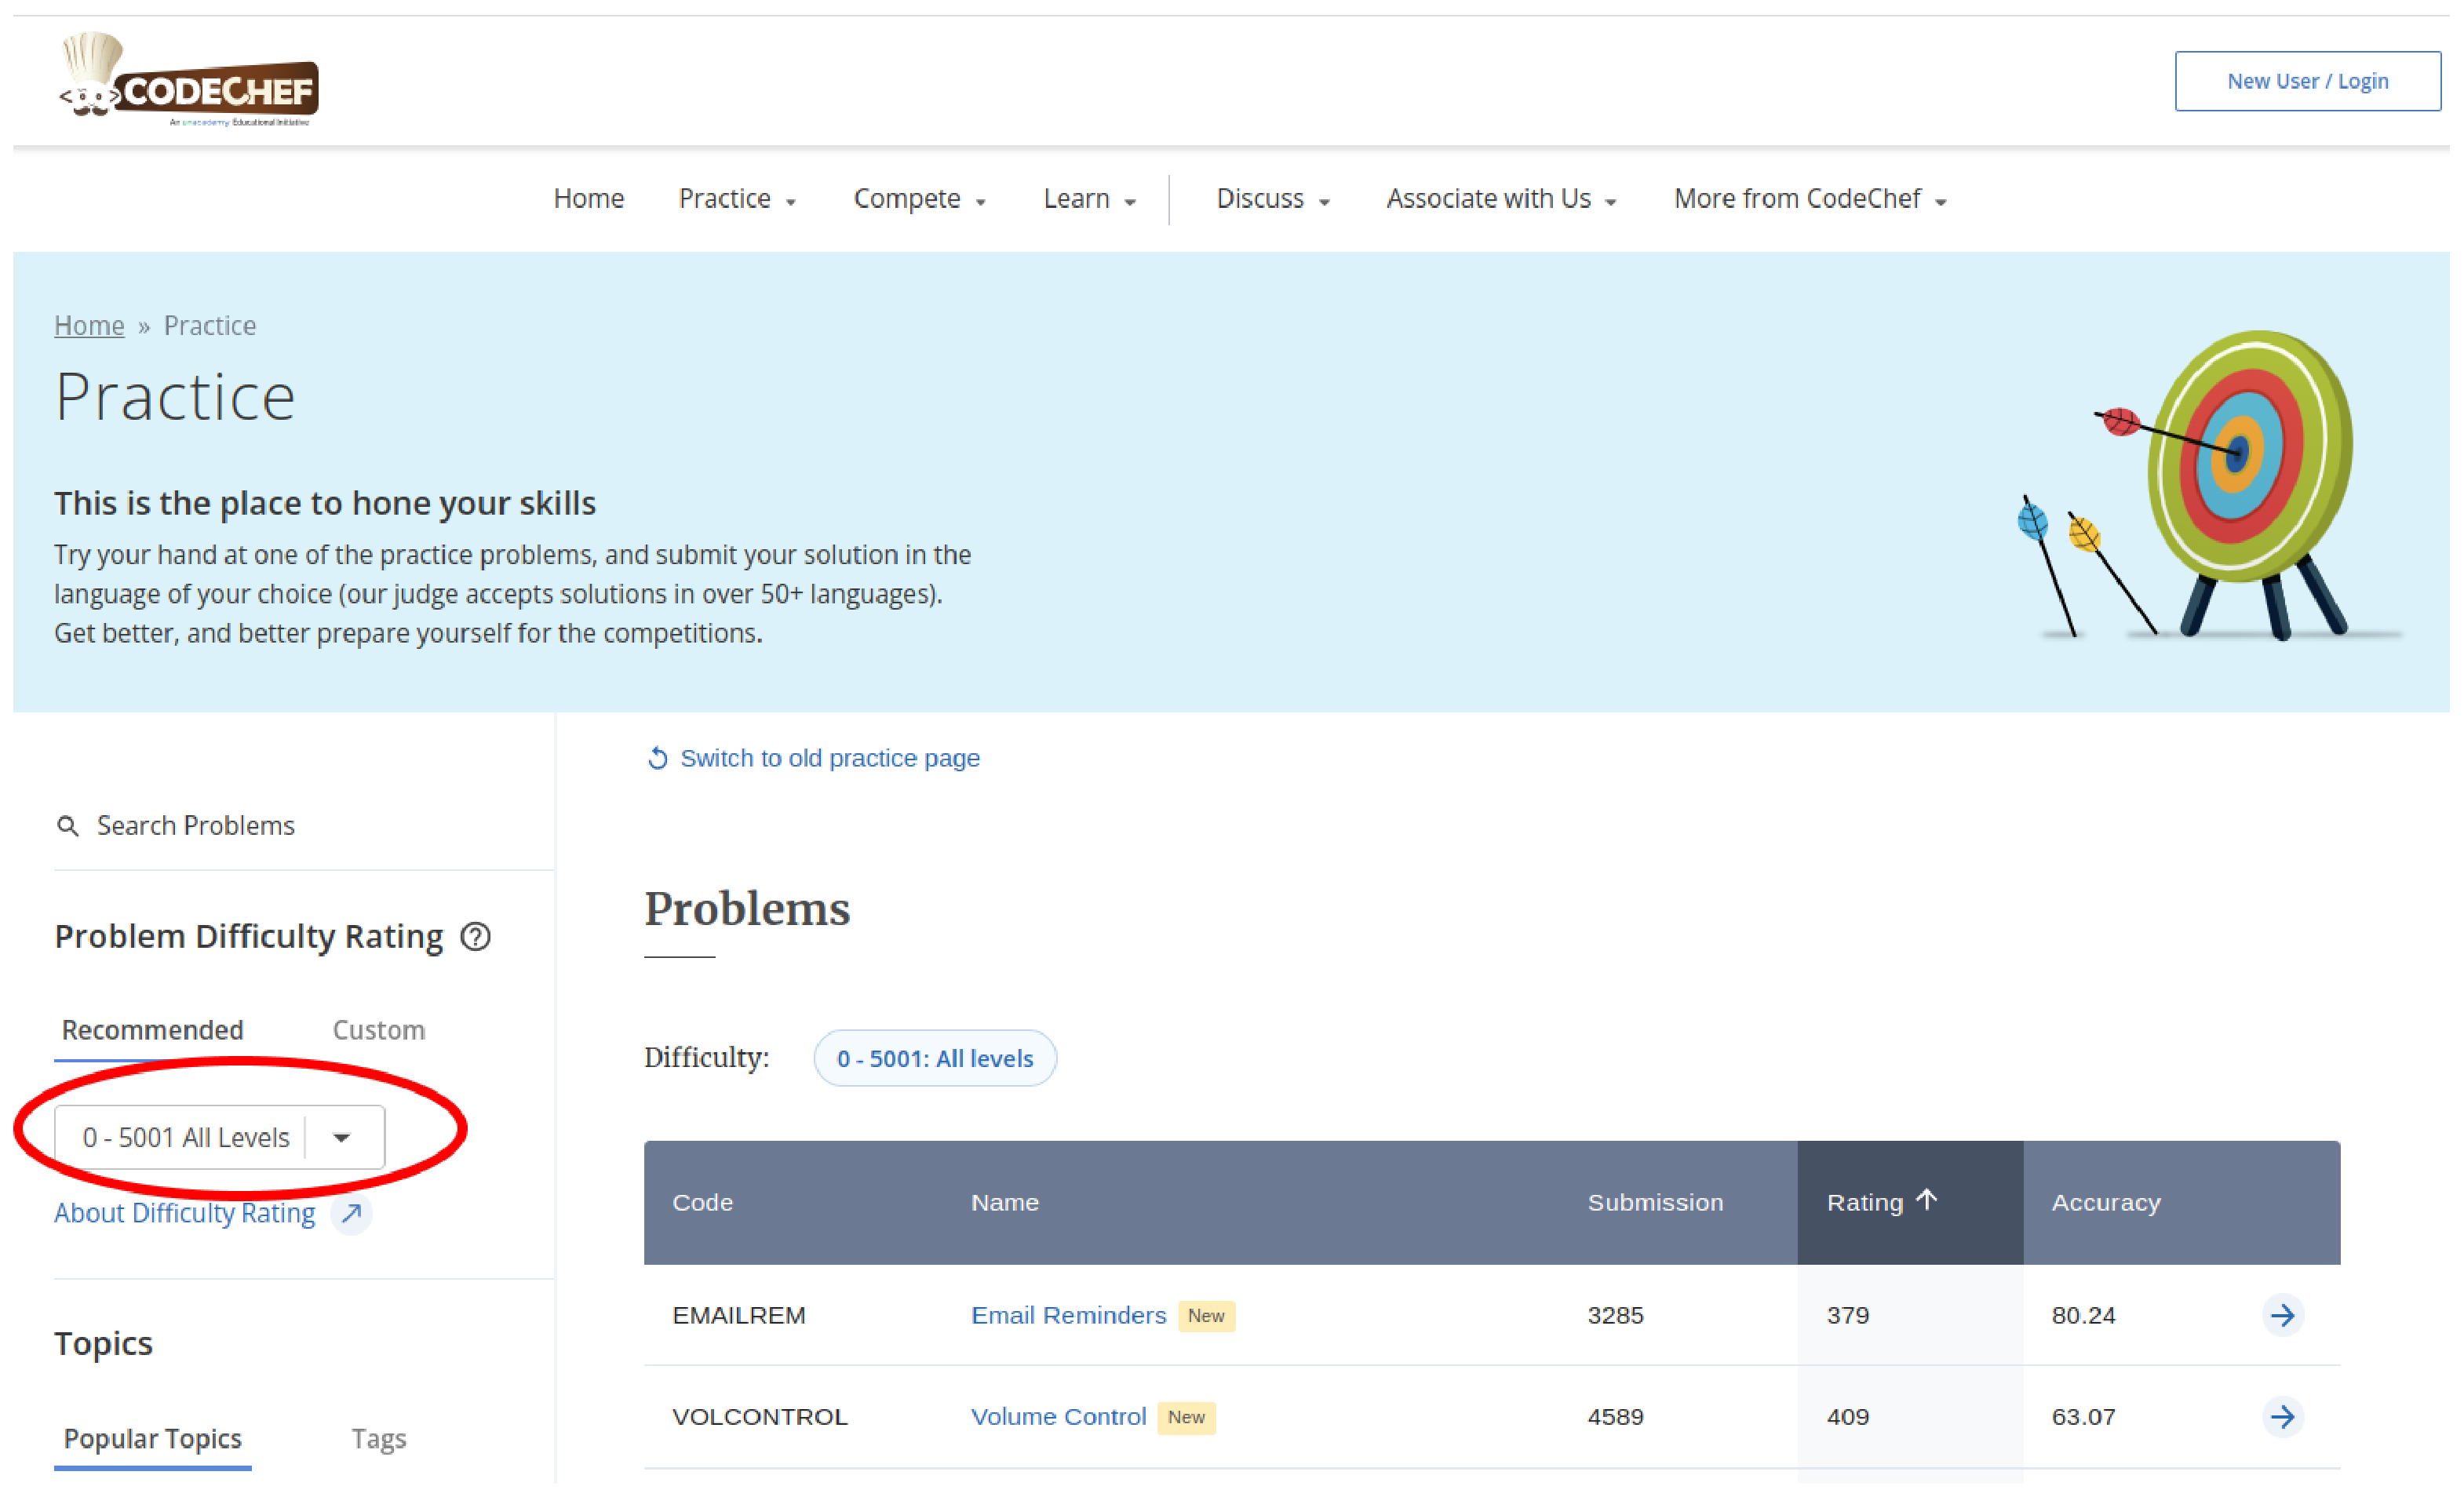
\includegraphics[keepaspectratio=true,scale=0.3]{figuras/code_chef_1.eps}
    \label{fig:code_chef_1}
\end{figure}

\begin{figure}[H]
    \centering
    \caption{Code Chef — Número de problemas}
    
\includegraphics[keepaspectratio=true,scale=0.3]{figuras/code_chef_2.eps}
    \label{fig:code_chef_2}
\end{figure}

Para o levantamento do número de problemas no Google's coding competition foram separados 3 categorias diferentes, correspondentes aos 3 eventos anuais do Google: Code Jam, KickStart e HashCode. Na categoria Code Jam existem 8 rounds diferentes, dentre eles rounds de prática, classificatórios e os oficiais. O número de problemas das finais variam de 5 a 6 problemas, enquanto nos demais rounds varia de 3 a 4 problemas, como até hoje foram efetuados 4 competições, começando em 2018, foi estimado o total de 120 problemas para essa categoria. Na categoria KickStart são 8 rounds, cada round contendo 3 problemas. A competição teve início em 2018 totalizando 4 edições, com isso o número de problemas é 96. Por fim na categoria HashCode há apenas 2 problemas por edição, 1 problema do round classificatório e 1 do round final, totalizando 8 problemas nas 4 edições que se iniciaram em 2018.

Não foi possível fazer o levantamento do número de problemas na plataforma CodeBench, pelo fato dos problemas serem privados. A plataforma disponibiliza para professores a criação de turma, onde o acesso é controlado e por conta disso, não foi feita uma estimativa do número de problemas na plataforma.

Para o levantamento de questões no Sphere Online Judge, foi acessado  o menu de problemas. Nele foram localizadas 6 categorias: ``\textit{Classical}'', ``\textit{Chalenge}'', ``\textit{Partial}'', ``\textit{Tutorial}'', ``\textit{Riddle}'' e ``\textit{Basics}'', como demonstra a Figura \ref{fig:spoj}. Para o levantamento do número de questões foram acessadas cada uma das categorias, e o número de páginas por categoria foi contado. Com exceção da última página, as demais apresentam 50 problemas; portanto, para ter o total de problemas, foram contadas as páginas — exceto a última — e o resultado foi multiplicado por 50. Em seguida, foi adicionado o total de problemas da última página ao valor; na Tabela \ref{table:spoj_categories} são apresentadas as informações citadas observadas por categoria.

\begin{figure}[H]
    \centering
    \caption{Sphere Online Judge — Categorias de problemas}
    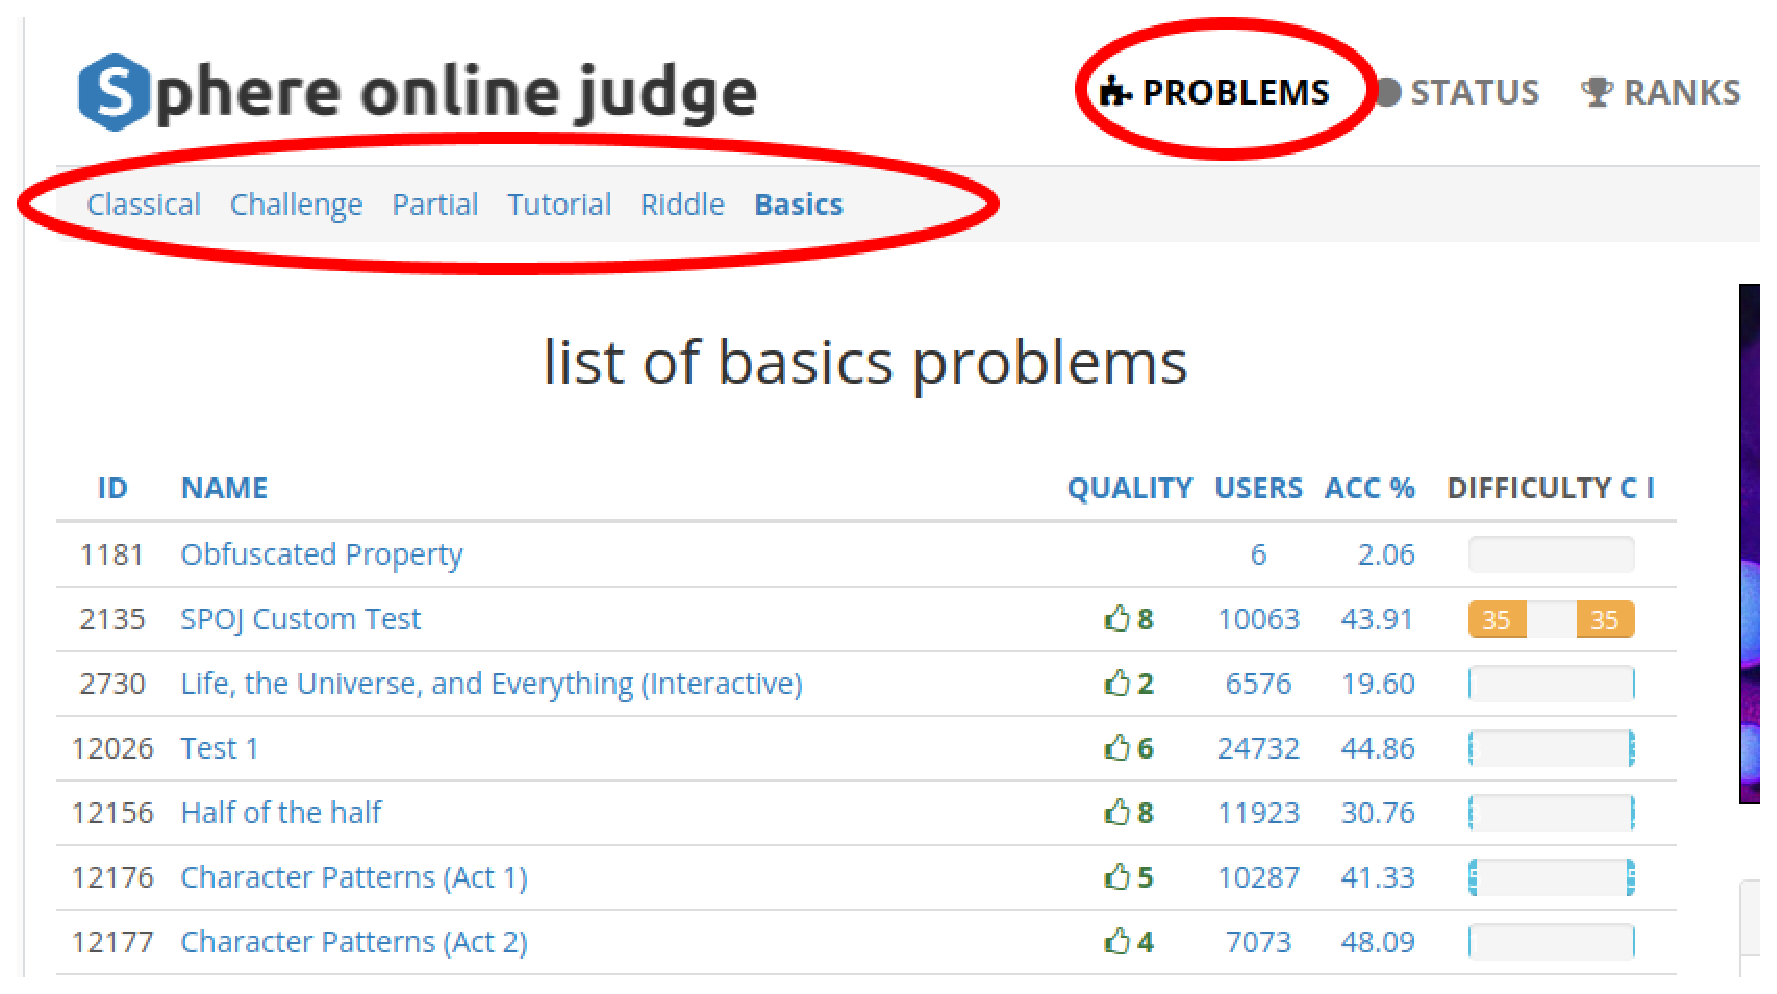
\includegraphics[keepaspectratio=true,scale=0.4]{figuras/spoj.eps}
    \label{fig:spoj}
\end{figure}

\begin{table}[ht]
    \caption[Caption for LOF]{Informações das categorias — Sphere Online Judge \footnotemark}
    \centering
    \label{table:spoj_categories}
\begin{tabular}{lll}
\rowcolor[HTML]{CBCEFB} 
Categoria & Número de páginas & Problemas na última página \\
Classical & 79                & 50                         \\
Chalenge  & 4                 & 10                         \\
Tutorial  & 28                & 49                         \\
Partial   & 1                 & 35                         \\
Basics    & 7                 & 3                         
\end{tabular}
\end{table}
\footnotetext{Data da observação: 05/04/2022}

Os demais juízes onlines possuem alguma forma de apresentar todos os problemas separados por páginas com um valor fixo de problemas em cada uma delas. Com isso, o método para contagem nos demais sites foi: o valor do número de problemas por página é multiplicado pelo total de páginas com exceção da página final, e depois, o número de problemas na última página é adicionado ao valor total. Na figura \ref{fig:hackerearth_numero_problemas} é possível observar esse padrão na plataforma Hackerearth, que apresenta 77 páginas e um total de 20 problemas em cada; sem contar com a última página, é possível estimar o número de problemas em 1520.
 
\begin{figure}[H]
    \centering
    \caption{Hackerearth — Número de problemas}
    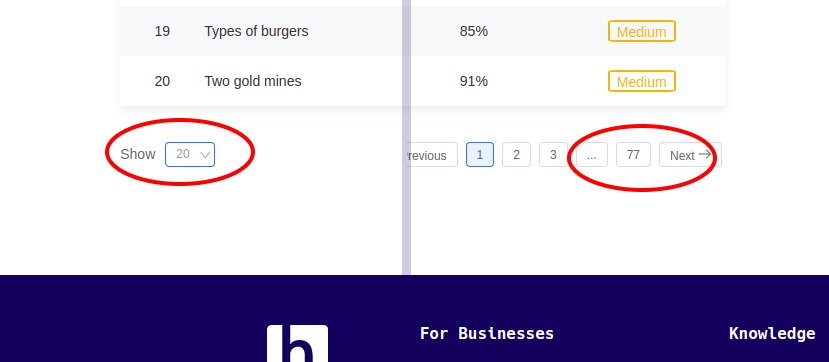
\includegraphics[keepaspectratio=true,scale=0.45]{figuras/hackerearth_numero_problemas.png}
    \label{fig:hackerearth_numero_problemas}
\end{figure}

Na Tabela \ref{table:problemas_por pagina} o levantamento dessas informações para os demais juízes é representado nas colunas: ``Problemas por página'', ``Total de páginas'' e ``Problemas na última página''; com essas informações é possível fazer uma estimativa do total número de problemas em cada uma das plataformas disponíveis na Tabela.

\begin{table}[ht]
    \caption{Coleta do número de problemas por página}
    \centering
    \label{table:problemas_por pagina}
\begin{tabular}{llll}
\rowcolor[HTML]{CBCEFB} 
Juíz online &
  \begin{tabular}[c]{@{}l@{}}Problemas \\ por página\end{tabular} &
  \begin{tabular}[c]{@{}l@{}}Total \\ de páginas\end{tabular} &
  \begin{tabular}[c]{@{}l@{}}Problemas \\ na última página\end{tabular} \\
Hackerearth      & 20  & 77 & 6  \\
PKU Judge Online & 100 & 31 & 54 \\
Neps Academy     & 16  & 67 & 13
\end{tabular}
\end{table}


\section{Arquitetura}
\label{sec:arquitetura}

A arquitetura escolhida para execução do GOJ foi a de micro-serviços, separando a aplicação em módulos com pequenos conjuntos de responsabilidades individuais. Além dos módulos desenvolvidos, foram utilizados os seguintes servições externos: serviço de filas, notificações e armazenamento. A Figura \ref{fig:arquitetura_goj} representa toda a arquitetura do projeto e os módulos desenvolvidos: ``Gamma Judge Admin'', ``Gamma Judge UI'', ``Gamma Judge API'' e ``Gamma Judge Tools''.

\begin{figure}[H]
    \centering
    \caption{Arquitetura geral GOJ}
    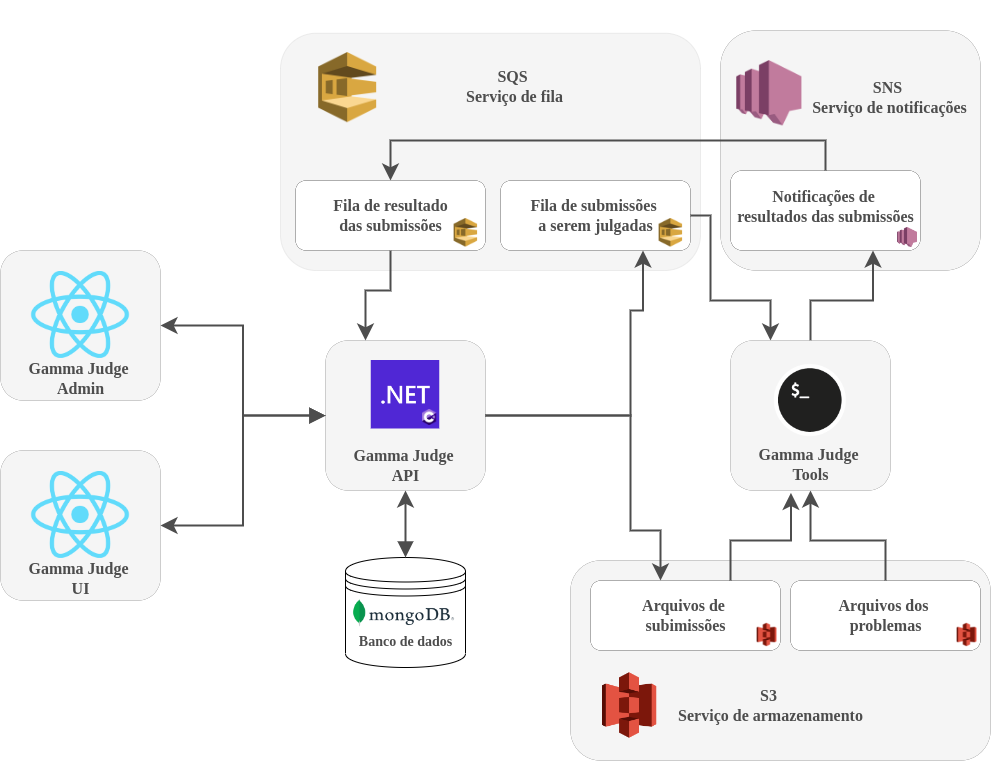
\includegraphics[keepaspectratio=true,scale=0.45]{figuras/arquitetura_goj.png}
    \label{fig:arquitetura_goj}
\end{figure}

Nessa seção serão abordadas as arquiteturas, tecnologias e os métodos utilizados para o desenvolvimento dos módulos. Também serão abordadas as ferramentas externas e serviços externos utilizados no desenvolvimento do projeto.

\subsection{Servições externos} 
\label{subsec:arquitetura_servicos_ext}

Na arquitetura do projeto, foram utilizados recursos do AWS Console\footnote{\url{https://aws.amazon.com/pt/console/}}, console que disponibiliza ferramentas diversas para a manutenção, processamento e armazenamento de aplicações na nuvem; além disso, existem serviços prontos que auxiliam o desenvolvimento de aplicações. No projeto GOJ, os serviços AWS que fazem parte da arquitetura são: Simple Queue Service (SQS), o Simple Notification Service (SNS) e o Simple Storage Service (S3).

O SQS consiste em um serviço online de filas, onde mensagens podem ser enviadas, lidas e consumidas. A ideia da utilização desse serviço é manter a consistência do funcionamento da aplicação em casos de intermitência ou erros do sistema. No projeto o serviço SQS é utilizado para que a comunicação entre o Gamma Judge API — que recebe as submissões do usuário — e o Gamma Judge Tools — que julga as submissões lidas da fila — seja consistente. No caso onde o sistema apresente falhas pontuais para julgar as submissões, como: falta de memória na máquina, ou até mesmo inatividade do serviço, a mensagem não será consumida ou ficará no sistema de filas até que seja; isso entrega uma maior consistência, pois, em caso de inatividade ou intermitência do Gamma Judge Tools o envio de submissões não será comprometido.

Já o SNS é um serviço de notificações, a ideia dele é que uma mensagem enviada possa ser distribuída para outros serviços. Sua utilização no GOJ é para notificar que uma submissão foi julgada, a notificação é enviada através de um tópico SNS e os serviços inscritos nesse tópico recebem a mensagem. A ``Fila de resultados das submissões'' é inscrita no tópico SNS ``Notificações de resultados das submissões'', como demonstrado na Figura \ref{fig:arquitetura_goj}, e todas as mensagens enviadas nesse tópico são enviadas para a fila, para que os resultados possam ser consumidos e apresentados ao usuário final.

Por fim, o S3 é um serviço de armazenamento de arquivos. Ele é utilizado para ler e armazenar os arquivos enviados das submissões e os arquivos necessários para julgar as questões. A utilização de um serviço de armazenamento permite que os arquivos sejam acessados por mais de um módulo da aplicação, como acontece na arquitetura do projeto.

\subsection{Gamma Judge API} 
\label{subsec:arquitetura_judge_api}

O módulo Gamma Judge API é responsável por fazer uma ponte de comunicação com a \textit{interface}, disponibilizando as informações armazenadas e recebendo arquivos para serem julgados pelo juiz eletrônico. Além disso, é responsabilidade desse módulo, processar as informações dos resultados das submissões. Na Figura \ref{fig:arquitetura_goj_api} são demonstrados os fluxos descritos, e as interações com a \textit{interface} e os serviços externos.

\begin{figure}[H]
    \centering
    \caption{Arquitetura — Gamma Judge API}
    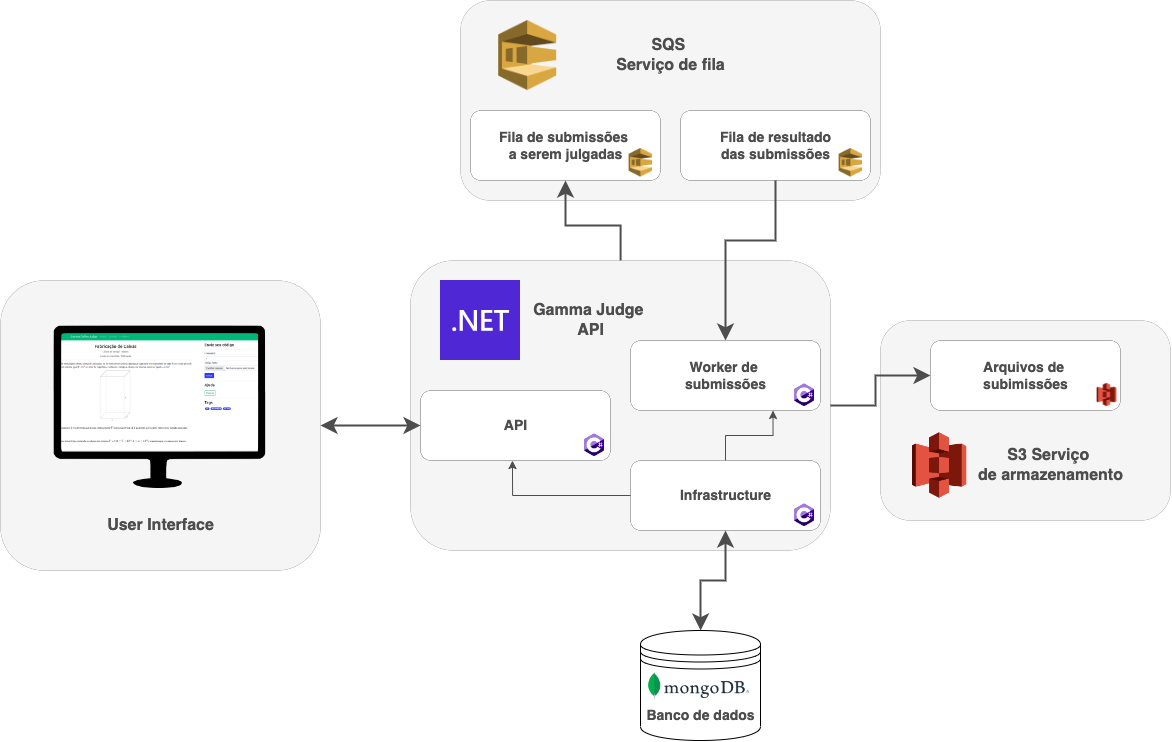
\includegraphics[keepaspectratio=true,scale=0.35]{figuras/arquitetura_goj_api.png}
    \label{fig:arquitetura_goj_api}
\end{figure}

Como demonstrado, o sistema faz o uso de 2 serviços externos, são eles: SQS e S3. O SQS é utilizado para receber as informações dos resultados das submissões e para o envio de submissões a serem julgadas. Já o serviço S3 é utilizado para o armazenamento dos arquivos de submissões. 

O Gamma Judge API se divide em 3 grandes partes, a ``API'', o ``Worker de submissões'' e a ``Infrastructure'', como demonstrado na Figura \ref{fig:arquitetura_goj_api}. A ``API'' é responsável pela comunicação externa, recebendo e enviando informações para uma interface de usuário; O ``Worker de submissões'' é um \textit{background service} que processa as submissões recebidas; e a ``Infrastructure'' é uma abstração dos serviços externos, ela se comunica diretamente com o banco de dados e os serviços SQS e S3, disponibilizando funções para os demais módulos utilizarem.

Para o envio de uma submissão a API recebe um arquivo, contendo o código-fonte enviado, as configurações, como linguagem e compilador que serão utilizados e, as informações do problema, que determinarão quais são as entradas e saídas esperadas da submissão que será julgada. Após recebidas, as informações da submissão são armazenadas no banco de dados, o arquivo é enviado para o S3 com um identificador único, que associa aquele arquivo àquela submissão e, as informações são enviadas para a ``Fila de submissões a serem julgadas'' no SQS, posteriormente um juiz eletrônico é responsável por reunir esses dados e julgar o problema. Após julgada, o resultado da submissão é enviado para a fila SQS ``Fila de resultado das submissões'', onde os resultados são processados e atualizados no banco de dados.

Esse sistema foi desenvolvido utilizando o .NET Frameweork com C\# de linguagem de programação principal. O banco de dados é um MongoDB, para o armazenamento das informações de questões, eventos e submissões. A comunicação com a ``User interface'' é feita via protocolo HTTP, para o recebimento e disponibilização de informações. Para melhora da compatibilidade e facilidade com a entrega desse sistema foi utilizado a ferramenta Docker, um sistema de virtualização que permite que o projeto seja executado em qualquer plataforma que suporte a ferramenta.

\subsection{Gamma Judge Tools} 
\label{subsec:arquitetura_judge_tools}

% Responsável por executar arquivos em uma linguagem de programação, com uma lista de entradas e saídas esperadas. Além disso, é responsabilidade desse módulo retornar ao usuário um veredito de execução, de acordo com um tempo de execução limite, limite de memória permitido e saídas esperadas. 

O Gamma Judge Tools é o módulo responsável por julgar submissões e retornar o veredicto. Esse módulo realiza o papel de um juiz eletrônico e funciona com o auxílio dos serviços externos citados na Subseção \ref{subsec:arquitetura_servicos_ext}. Os serviços externos utilizados nesse módulo são: SQS, SNS e S3, como demonstrado na Figura \ref{fig:arquitetura_goj_tools}.

\begin{figure}[H]
    \centering
    \caption{Arquitetura — Gamma Judge Tools}
    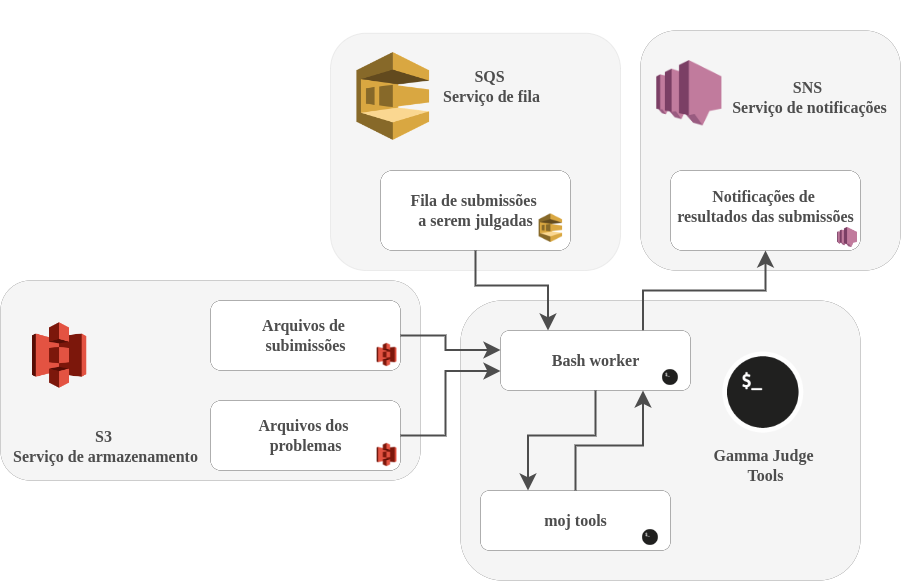
\includegraphics[keepaspectratio=true,scale=0.45]{figuras/arquitetura_goj_tools.png}
    \label{fig:arquitetura_goj_tools}
\end{figure}

O sistema foi desenvolvido em linguagem de programação bash e possui um \textit{worker} para consumir as submissões. Cada submissão recebida possui as informações do problema correspondente: linguagem, identificador do problema e o identificador do arquivo armazenado no S3. Reunidas as informações o sistema executa o arquivo de submissões em uma lista de testes; o resultado da execução é enviado para uma notificação SNS, informando o veredicto da submissão, AC, WA, TLE, MLE ou RTE \footnote{Ver em: \ref{sec:juizesOnline}}. Em caso de falha do juiz na execução, a mensagem não é consumida, e volta para a fila SQS para ser lida novamente.

Por esse módulo ser um serviço separado do Gamma Judge API, não é necessária sua exposição a \textit{web}, além disso, as filas SQS realizam o controle de concorrência caso mais de um consumidor esteja acessando esse recurso, possibilitando uma maior facilidade para escalonar o sistema. Ou seja, caso seja necessário mais poder de processamento ou paralelismo para julgar as questões, basta rodar o Gamma Judge Tools em uma máquina adicional diferente, sem se preocupar com a concorrência entre os consumidores e a fila SQS. 

\subsection{Gamma Judge UI e Gamma Judge Admin} 
\label{subsec:arquitetura_judge_ui}

O Gamma Judge UI é a interface de usuário que se comunica com a API, recebendo e enviando informações. Ela recebe as informações dos problemas, eventos e submissões, e envia os códigos para serem processados. O Gamma Judge Admin tem um comportamento similar, porém as informações enviadas são para edição, criação e exclusão de problemas e eventos. 

Ambos os módulos foram desenvolvidos em Node JS, com Typescript de linguagem principal. Nos projetos foram utilizados \textit{Node Packages}, bibliotecas externas que facilitam o desenvolvimento web (Ver em \ref{sec:desenvolvimentoWEB}). Das bibliotecas utilizadas, as principais foram: \textit{React Bootstrap}\footnote{https://react-bootstrap.github.io/}, que disponibiliza componentes, como botões, textos e tabelas, \textit{React Router}\footnote{https://v5.reactrouter.com/web/guides/quick-start}, que disponibiliza recursos para navegação e \textit{React LaTEX}\footnote{https://www.npmjs.com/package/react-latex}, que permite a renderização de elementos HTML e LaTEX.

O Gamma Judge UI é responsável por renderizar elementos não textuais, como fórmulas, imagens e elementos necessários para a visualização das informações de um problema. As informações são recebidas em texto, HTML ou LaTEX, da API, e o sistema é responsável por transformar essas informações em elementos visuais como fórmulas, tabelas ou imagens. Para isso, o pacote \textit{React LaTEX} é utilizado, ele permite a inserção de trechos em LaTEX ou HTML para a visualização na página WEB.

% Background service
%  https://docs.microsoft.com/pt-br/aspnet/core/fundamentals/host/hosted-services?view=aspnetcore-6.0&tabs=visual-studio

% TODO

% \subsection{Levantamento das funcionalidades dos juízes}
% \label{subsec:levantamento_funcionalidades}

% Nessa subseção será abordada a maneira onde o levantamento das funcionalidades existentes em cada um dos juízes online foi realizada. As observações de cada um dos juízes foi efetuada de maneira diferente, apesar de a abordagem ter sido similar em aluns.

% As funcionalidades do site \textit{Online Judge} foram levantadas simplesmente navegando pelo site, enviando problemas olhando a resposta e buscando por tutoriais e ferramentas adicionais no próprio site. O site possui links para ferramentas externas como \textit{uDebug}\footnote{\url{https://www.udebug.com/UVa/}}, plataforma que auxilia a solução dos problemas disponibilizado um código correto para comparação de entradas e saídas, e o \textit{uHunt} uma plataforma direcionada para o site \textit{Online Judge} que deixa a resolução de questões mais iterativa, mostrando estatísticas dos problemas resolvidos e separando as questões em categorias. 

% Para o levantamento das funcionalidades no site \textit{PKU Online Judge}, foi feita uma navegação no site e acessando as funcionalidades foi possível coletar algumas informações. Ao enviar uma questão, e é possível perceber que o site aceita algumas linguagens e compiladores como mostrado na Figura \ref{fig:pku_2}, porém não foi possível receber o veredicto de uma questão enviada, pois no dia 5 de abril as 11:43, horário onde o teste foi feito, o site retornava um erro ao enviar a questão;

% Já no \textit{Codeforces}, as funcionalidades foram observadas navegando e enviando questões.  O foco do site está em competições, e ocorrem competições semanalmente. Além disso, a maioria dos problemas possui tutoriais e os códigos e soluções de outras pessoas são abertos.


% \section{Levantamento de requisitos}
% \label{sec:levantamentoDeRequisitos}

% Antes e durante o desenvolvimento do GOJ, foi necessário realizar um levantamento de requisitos. Essa etapa é importante para obter detalhadamente os recursos que englobam a aplicação \cite{young2002recommended}.

% Foram utilizadas algumas técnicas para o levantamento de requisitos. Abordagens Discutidas por \citeonline{young2002recommended}. Semanalmente, foram feitas entrevistas para entendimento do sistema. Durante algumas dessas semanas, foram feitas prototipagens para assegurar o correto andamento do desenvolvimento.

% Os requisitos da aplicação levantados se dividem em três principais, descritos na Tabela \ref{table:reqGerais}:

% \begin{table}[ht]
%     \caption{Requisitos gerais}
%     \centering
%     \label{table:reqGerais}
%     \begin{tabular}{ |p{0.5cm}|p{3cm}|p{10cm}|  }
%         \hline
        
%         \textit{\textbf{Id}} & 
%         \textbf{Tópico} & 
%         \textbf{Requisito} \\
%         \hline
        
%         1 & 
%         Armazenamento   & 
%         É necessário armazenar um número limitado de questões e eventos das edições das maratonas UnB de programação, com atualização não frequente.  \\
%         \hline
        
%         2 & 
%         Juiz & 
%         O usuário deve conseguir enviar sua solução em código para ela ser julgada, retornando um veredicto de sua submissão.  \\ 
%         \hline
        
%         3 & 
%         Interface & 
%         O usuário deve conseguir ter acesso aos problemas e eventos.  \\
%         \hline
%     \end{tabular}

% \end{table}

% Os requisitos citados na Tabela \ref{table:reqGerais} englobam a aplicação. Contudo, são requisitos não detalhados e não específicos; esse fator, pode gerar ambiguidade ou incompletude para os mesmos, como salienta ``[\dots] Cada requisito deve ser necessariamente, verificável, atingível, inequívoco, completo, consistente, rastreável, conciso, livre de implementação[\dots]''\footnote{\textit{``[\dots] Each requirement should be necessary, verifiable, attainable, unambiguous, complete, consistent, traceable, concise, implementation-free [\dots]''}} \cite[p.9, tradução nossa]{young2002recommended}.

% Com base do exposto os requisitos foram divididos em requisitos menores e mais específicos. Com isso, mais detalhes foram listados na busca de uma maior completude e clareza. Os requisitos menores serão descritos nas seguintes subseções: \nameref{subsec:storage}, \nameref{subsec:juiz} e \nameref{subsec:ui}.

% \subsection{Armazenamento das questões e eventos}
% \label{subsec:storage}

% Esse módulo do sistema é responsável pelo armazenamento das questões, enunciados e eventos. Essa parte do \textit{software} deve ser responsável por disponibilizar essas informações para os outros módulos. Na Tabela \ref{table:reqArmazenamento} se encontram os requisitos levantados dessa parte da aplicação:

% \begin{table}[ht]
%     \caption{Requisitos de armazenamento}
%     \centering
%     \label{table:reqArmazenamento}
%     \begin{tabular}{ |p{0.6cm}|p{3cm}|p{10cm}|  }
%         \hline
        
%         \textbf{Id} & 
%         \textbf{Tópico} & 
%         \textbf{Requisito} \\
%         \hline
        
%         1.1 & 
%         Armazenamento   & 
%         As questões devem possuir título, enunciado, tempo limite de execução, limite de memória utilizado pelo programa, lista de rótulos que categorizam o problema, ID predefinido para localização das questões e identificação e lista de entradas e saídas de teste. \\
%         \hline
        
%         1.2 & 
%         Armazenamento & 
%         Os eventos devem possuir uma data, que identifica quando o evento aconteceu, um nome e uma lista de problemas, tal como o rótulo do problema naquele evento ex: “Questão A”  \\ 
%         \hline
        
%         1.3 & 
%         Armazenamento & 
%         O sistema precisa conseguir fazer uma busca por nome, rótulo ou evento.  \\
%         \hline
%     \end{tabular}

% \end{table}

% Os requisitos citados na Tabela \ref{table:reqArmazenamento} tem uma granularidade maior que os citados na Tabela \ref{table:reqGerais}. Com isso, o desenvolvimento das funcionalidades se torna mais preciso, evitando que expressões genéricas gerem ambiguidades com as necessidades da aplicação.

% \subsection{Juiz das questões}
% \label{subsec:juiz}

% Esse módulo do sistema é responsável por julgar um problema. Ao enviar um código para ser julgado o sistema deve processá-lo, rodá-lo na linguagem escolhida e comparar com as soluções esperadas. Na Tabela \ref{table:reqJuiz}, estão os requisitos levantados desse módulo.

% \begin{table}[ht]
%     \caption{Requisitos do juiz}
%     \centering
%     \label{table:reqJuiz}
%     \begin{tabular}{ |p{0.6cm}|p{2cm}|p{11cm}|  }
%         \hline
        
%         \textbf{Id} & 
%         \textbf{Tópico} & 
%         \textbf{Requisito} \\
%         \hline
        
%         2.1 & 
%         Juiz & 
%         O sistema deve receber arquivos ou textos contendo códigos em linguagens de programação pré, definidas. \\ 
%         \hline
        
%         2.2 & 
%         Juiz & 
%         As principais linguagens suportadas pelo sistema devem ser C, C++, Java e Python.  \\
%         \hline
        
%         2.3 & 
%         Juiz & 
%         Os arquivos/textos recebidos devem ser executados com uma lista de entradas e saídas esperadas. \\
%         \hline
        
%         2.4 & 
%         Juiz & 
%         O sistema deve conseguir saber a memória e tempo utilizados para execução do programa; dependendo da memória e do tempo de execução do código o veredito pode mudar de aceito para não aceito. \\
%         \hline
%     \end{tabular}
% \end{table}

% Os requisitos citados na Tabela \ref{table:reqJuiz} correspondem ao módulo que julgará os códigos enviados pelos usuários. Os vereditos retornados podem ser AC, WA, TLE o MLE (\ref{sec:juizesOnline}).

% O comportamento desse módulo é o comportamento de um juiz eletrônico. Com isso essa parte do sistema se assimila bastante ao BOCA, sistema desenvolvido para realização de maratonas de programação \cite{de2004boca}; além disso, ele também é utilizado em disciplinas de programação na graduação \cite{francisco2016juiz}.

% \subsection{\textit{Interface} de usuário}
% \label{subsec:ui}

% Esse módulo do sistema corresponde a parte gráfica da aplicação. Nele, as informações dos outros módulos ficam visíveis para o usuário; portanto os requisitos presentes nesse módulo foram requisitos visuais, que estão descritos na Tabela \ref{table:reqInterface}:

% \begin{table}[ht]
%     \caption{Requisitos da interface}
%     \centering
%     \label{table:reqInterface}
%     \begin{tabular}{ |p{0.6cm}|p{3cm}|p{10cm}|  }
%         \hline
        
%         \textbf{Id} & 
%         \textbf{Tópico} & 
%         \textbf{Requisito} \\
%         \hline
        
%         3.1 & 
%         Interface   & 
%         As informações das questões devem estar disponíveis ao usuário, podendo conter formulas matemáticas e imagens. \\
%         \hline
        
%         1.2 & 
%         Armazenamento & 
%         Os eventos devem ser apresentados ao usuário de maneira organizada, com a lista dos respectivos problemas dos eventos.  \\ 
%         \hline
        
%         1.3 & 
%         Armazenamento & 
%         As informações de dicas e tutoriais das questões dever ser escondidas do usuário e disponíveis apenas se o usuário optar por elas.  \\
%         \hline
%     \end{tabular}

% \end{table}

% Os requisitos na Tabela \ref{table:reqInterface} descrevem como a \textit{interface} deve ser. Ela se assemelha a juízes \textit{onlines} presentes hoje, porém um foco direcionado para essa \textit{interface} é ser amigável para estudantes iniciantes em programação.